\documentclass[a4paper, 12pt]{article}
\usepackage[T1]{fontenc}
\usepackage[utf8]{inputenc}
\usepackage[english]{babel}
\usepackage{graphicx}
\usepackage{minted}
\usepackage{graphicx}
\usepackage{subcaption}
%\usepackage[hidelinks]{hyperref}
%\usepackage{hyperref}
%\usepackage{float}
\usepackage{setspace}
%\usepackage{amsfonts}
%\usepackage[nottoc,numbib]{tocbibind}
%\usepackage{amsmath}
%\numberwithin{equation}{section}


%\DeclareMathOperator*{\argmax}{arg\,max}

\onehalfspacing

\begin{document}

\title{Flatland Challenge}
\author{G. Berselli, M. M. L. Pulici}
\date{August 29, 2021}
\maketitle
\begin{center}
	\fbox{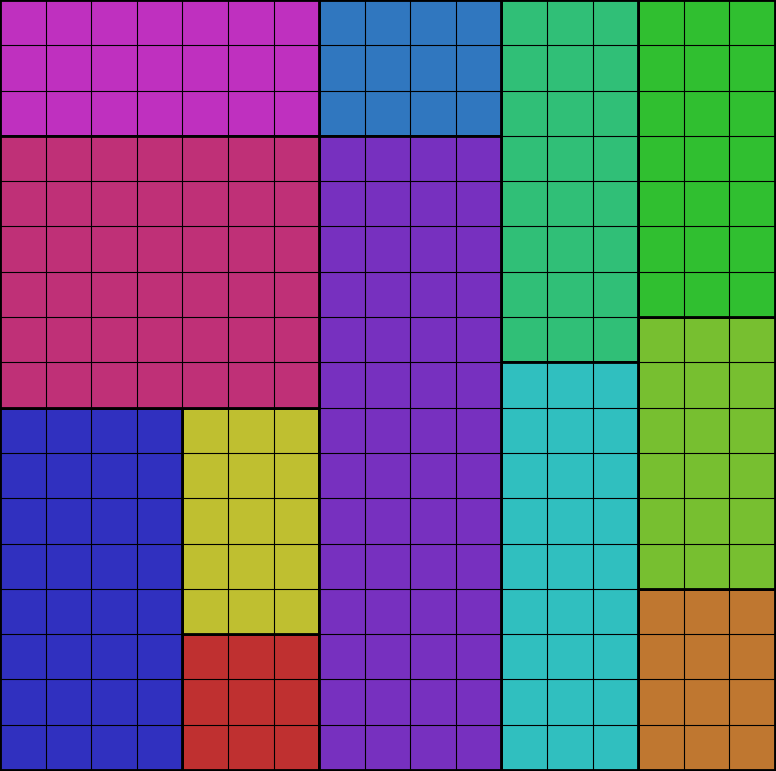
\includegraphics[width=0.618\textwidth]{Images/cover.png}}
\end{center}


\clearpage

\tableofcontents

\clearpage

\listoffigures

\clearpage


\section{Introduction}

\clearpage
\section{Modelling}


\subsection{Variables}

Each instance comes with 4 parameters describing the chip configuration:
\begin{itemize}
	\item \verb+chip_w+: the width of the chip;
	\item \verb+n+: the number of blocks to fit on the chip;
	\item \verb+inst_x+: a list containing the ordered widths of the blocks;
	\item \verb+inst_y+: a list containing the ordered heights of the blocks.
\end{itemize}
In addition, 3 auxiliary variables are created:
\begin{itemize}
	\item \verb+min_index+: the index of the smallest block (see Section \ref{sec:symmetry});
	\item \verb+min_h+: the minimum possible height of the chip (see Section \ref{sec:improvements});
	\item \verb+max_h+: the maximum possible height of the chip (see Sections \ref{sec:improvements}).
\end{itemize}
The results of the various solving procedures consists in 3 variables:
\begin{itemize}
	\item \verb+chip_h+: the height of the chip;
	\item \verb+bl_x+: a list containing the ordered horizontal positions of the bottom left corners of the blocks;
	\item \verb+bl_y+: a list containing the ordered vertical positions of the bottom left corners of the blocks.
\end{itemize}


\subsection{Constraints}

Given the problem to fit all blocks into the chip, the first obvious constraint is that of not making the blocks fall out of the chip. This is quite easy: it is sufficient to impose that, for every block \verb|k|:
\begin{itemize}
	\item \verb|bl_x[k] > 0|;
	\item \verb|bl_x[k] + inst_x[k] <= chip_w|;
	\item \verb|bl_y[k] > 0|.
\end{itemize}

The next step is to impose a non-overlapping constraint between each block pair. In order to do that, the basic idea is to cycle through all the blocks and to check that the distance between every bottom left corner pair is at least equal ti the dimension of the block in one direction. More practically, the following four constraints are inserted disjunctively for every pair of blocks \verb|k| and \verb|l|:
\begin{itemize}
	\item \verb|bl_x[k] + inst_x[k] <= bl_x[l]|;
	\item \verb|bl_y[k] + inst_y[k] <= bl_y[l]|;
	\item \verb|bl_x[l] + inst_x[l] <= bl_x[k]|;
	\item \verb|bl_y[l] + inst_y[l] <= bl_y[l]|.
\end{itemize}


\subsection{Symmetry breaking}\label{sec:symmetry}

In order to eliminate symmetrical solutions, a simple symmetry breaking constraint is introduced. As shown in Fig. \ref{fig:solutions}, each solution has four symmetrical configurations, where the blocks are located in symmetrical positions with respect to an horizontal and/or a vertical central symmetry ax.

\begin{figure}
    \centering
    \begin{subfigure}[t]{0.45\textwidth}
        \centering
        \fbox{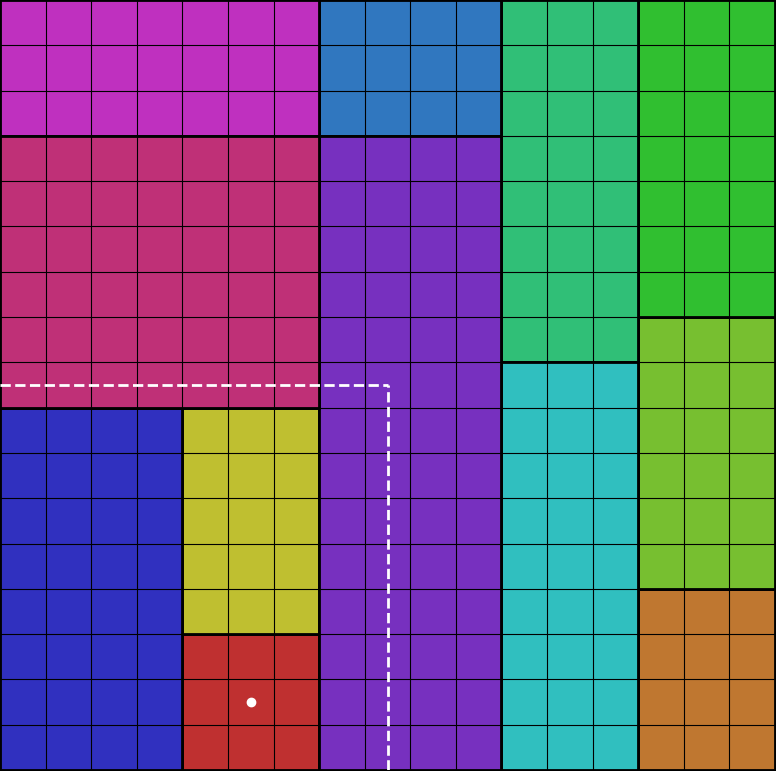
\includegraphics[width=\textwidth]{Images/symmetry-1.png}}
        \caption{Configuration 1.}
    \end{subfigure}
    \hfill
    \begin{subfigure}[t]{0.45\textwidth}  
        \centering 
        \fbox{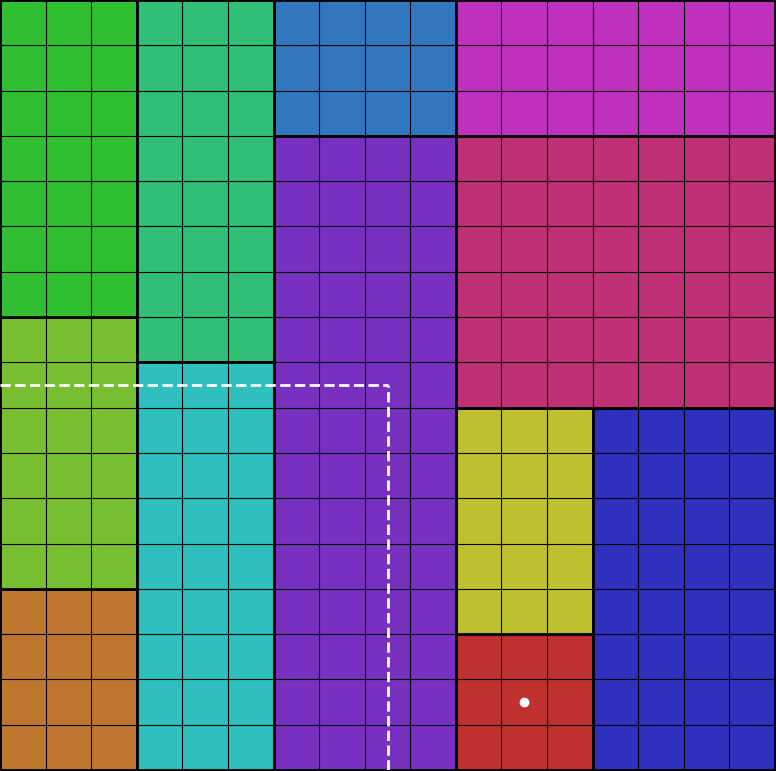
\includegraphics[width=\textwidth]{Images/symmetry-2.png}}
        \caption{Configuration 2.}
    \end{subfigure}
    \vskip\baselineskip
    \begin{subfigure}[t]{0.45\textwidth}   
        \centering 
        \fbox{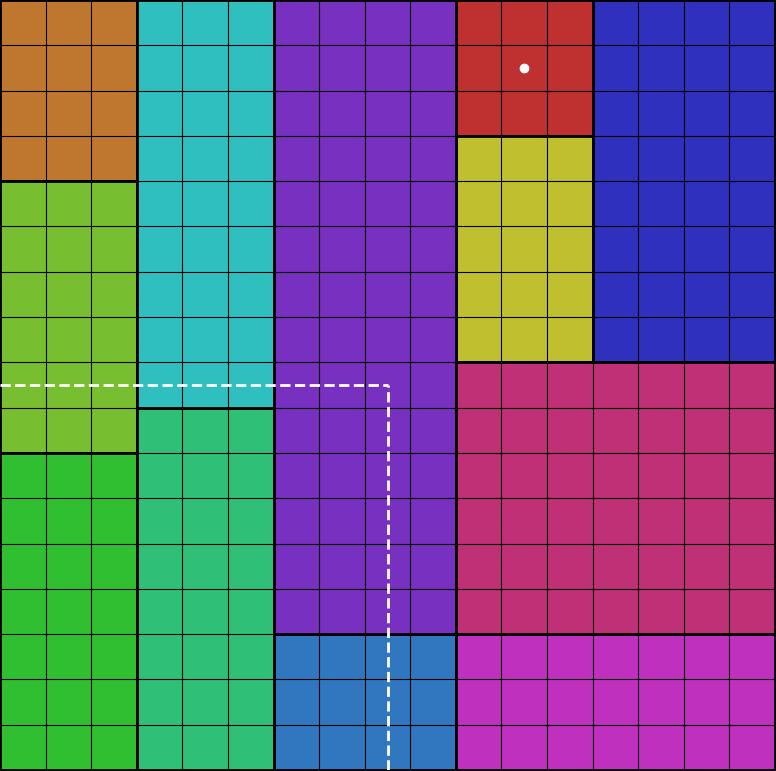
\includegraphics[width=\textwidth]{Images/symmetry-3.png}}
        \caption{Configuration 3.}
    \end{subfigure}
    \hfill
    \begin{subfigure}[t]{0.45\textwidth}   
        \centering 
        \fbox{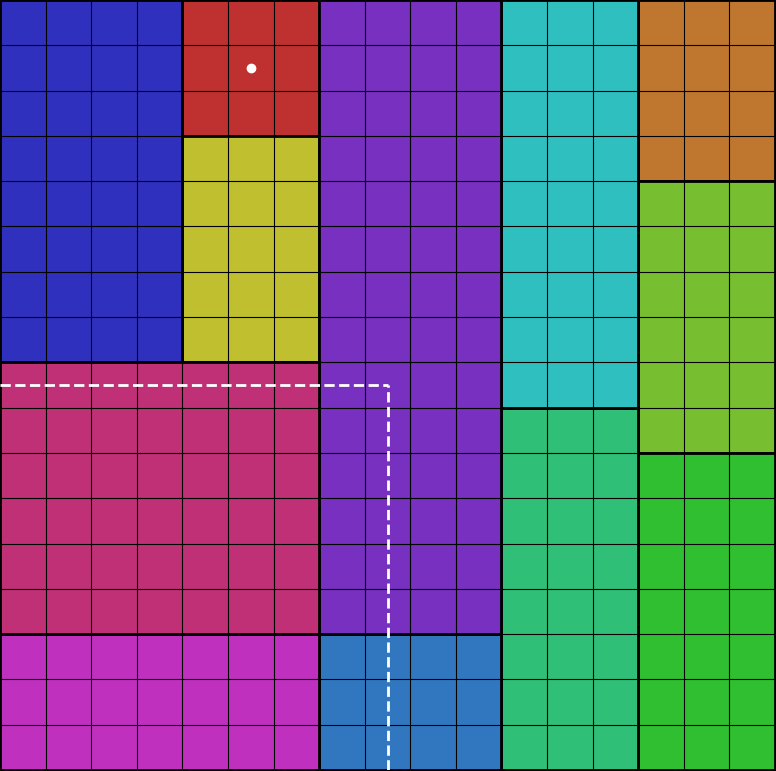
\includegraphics[width=\textwidth]{Images/symmetry-4.png}}
        \caption{Configuration 4.}
    \end{subfigure}
    \caption[Symmetrical configurations.]{Symmetrical configurations of Instance 10, with a white dot in the center of the smallest block and a dashed white line indicating the bottom left quadrant.}
    \label{fig:solutions}  
\end{figure}

In each of the configurations, the center of the smallest block is highlighted with a white dot and the bottom left quadrant is indicated by a dashed white line. It can be noted that, with the exception of very rare cases, the white dot lies in the highlighted quadrant in only one of the 4 symmetrical configurations. Therefore, the chosen symmetry breaking constraint consists in forcing the white dot to lie in the bottom left quadrant, i.e. adding the following conjunctive constraints, where \verb|min_index| is the index of the smallest block:
\begin{itemize}
	\item \verb|(2 * bl_x[min_index] + inst_x[min_index]) <= chip_w|;
	\item \verb|(2 * bl_y[min_index] + inst_y[min_index]) <= chip_h|.
\end{itemize}

\subsection{Rotation}


The next step is to implement rotations. Since the blocks are rectangular and nothing is known \emph{a priori} about whether they would wedge perfectly without gaps, it may be possible that the minimal height of the chip is obtained by rotating some of the blocks. For example, the difference between the two solutions for Instance 10 is shown in Fig. \ref{fig:rotations}. Even if in the given instances rotating does not actually reduce the chip height, it can still be observed that some blocks get rotated by the solver.

\begin{figure}
    \centering
    \begin{subfigure}[t]{0.45\textwidth}
        \centering
        \fbox{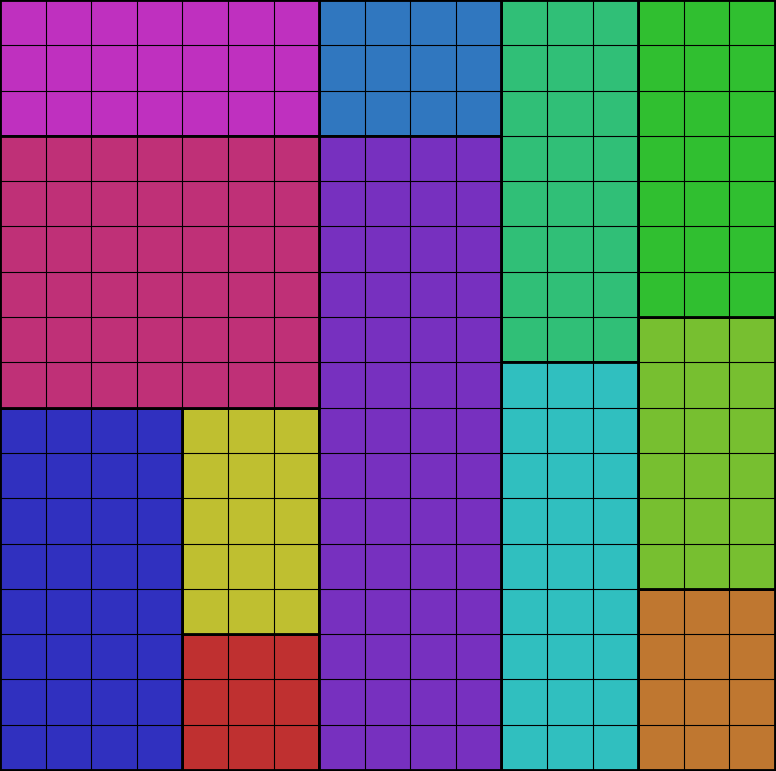
\includegraphics[width=\textwidth]{Images/cover.png}}
        \caption{Without rotations.}
    \end{subfigure}
    \hfill
    \begin{subfigure}[t]{0.45\textwidth}  
        \centering 
        \fbox{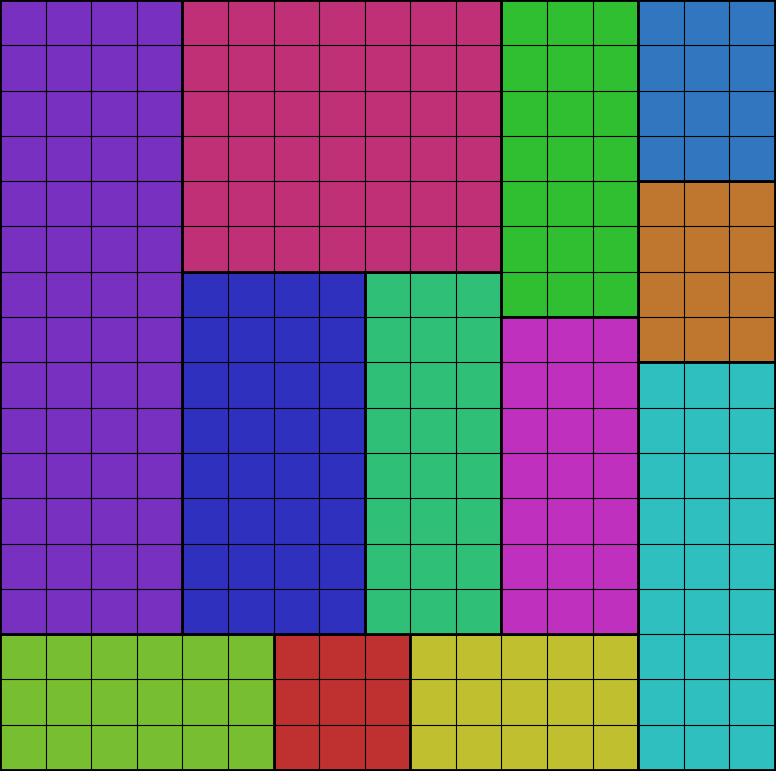
\includegraphics[width=\textwidth]{Images/rotated.png}}
        \caption{With rotations.}
    \end{subfigure}
    \caption[Solutions with and without rotations.]{Solutions of Instance 10 with and without enabled rotations.}
    \label{fig:rotations}  
\end{figure}

These rotations are handled differently in each implementation, but the basic idea is to offer both the normal and the rotated block to the solver and to impose an exclusive disjunction between the two orientations. In particular, it is useful to create a boolean vector of flags signalling whether each block is rotated (\verb|rotated|) and 2 auxiliary lists containing the actual dimensions of blocks (\verb|new_inst_x| and \verb|new_inst_y|). This way, since boolean values are by nature exclusive, the dimensions of each block \verb|k| can be linked to the respective boolean value with something similar to:
\begin{minted}{python}
new_inst_x[k] = inst_y[k] if rotated[k] == True else inst_x[k]
new_inst_y[k] = inst_x[k] if rotated[k] == True else inst_y[k]
\end{minted}



\subsection{Improvements}\label{sec:improvements}

The main improvement of the model consists in adding boundaries to \verb|chip_h|. The minimum height is fairly easy to evaluate, since in the best case scenario (i.e. if the blocks leave no gaps) \verb|min_h = total_area / chip_w|, where \verb|total_area| is calculated by simply adding up all the products of the blocks' dimensions. Computing the maximum height, on the other hand, is more subtle. A naive approach consists in simply adding all heights together, considering the worst case as that where all blocks are stacked vertically. This is of course a reasonable upper boundary, but, as the number of blocks increases, \verb|max_h| greatly overestimates the actual height.

A more clever solution can be reached with minimal preprocessing reasoning as follows. If blocks are ordered by height and width, the following code can be run:
\begin{minted}[linenos]{python}
chip_cumulative = chip_w
k = 0
heights = []
while k < len(inst):
    if inst[k][0] <= chip_cumulative:
        chip_cumulative -= inst[k][0]
        heights.append(inst[k][1])
        del inst[k]
    else:
        k += 1
max_h += max(heights)
\end{minted}

The reasoning is the following. The blocks' widths are compared with the free horizontal space (\verb+chip_cumulative+) and, if each block fits, the free space is decreased. When no more blocks fit on the line, the maximum height is taken among the located blocks and it is added to the total \verb|max_h|. The process is then repeated for the next lines as long as there are blocks left. This way, a much more optimistic, but strictly valid, \verb|max_h| is computed, as shown in Fig. \ref{fig:max_h}.

\begin{figure}
    \centering
        \fbox{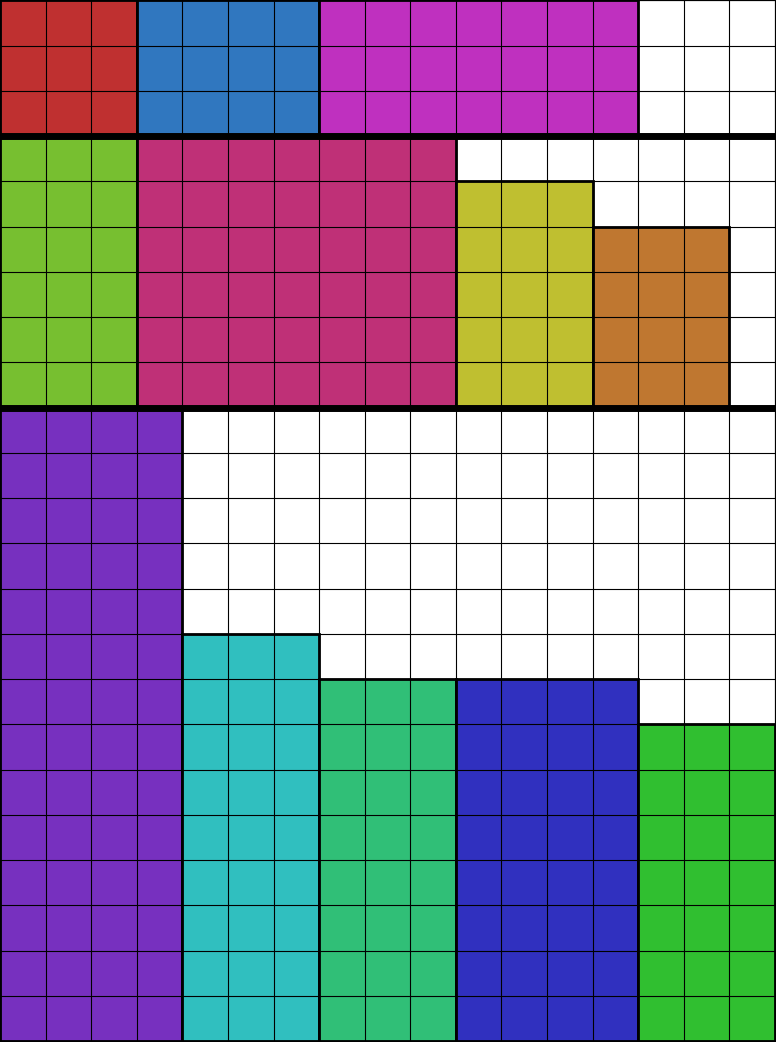
\includegraphics[width=\textwidth]{Images/max_h.png}}
        \caption[A graphical representation of the \texttt{max\symbol{95}h} algorithm.]{A graphical representation of the \texttt{max\symbol{95}h} algorithm for Instance 10.}
    \label{fig:max_h}  
\end{figure}


\clearpage

\end{document}



















